\chapter{经典力学}

\section{空间中的运动}
\subsection{平移与旋转}
\subsubsection{公式一览}\label{move-rot-formulas}
下表中的内容大部分来自于\cite{BibEntry2021Nov}。
\begin{longtable}{m{0.1\textwidth} m{0.38\textwidth}|m{0.1\textwidth} m{0.38\textwidth}}
\toprule
\multicolumn{2}{c|}{刚体平动} & \multicolumn{2}{c}{定轴转动} \\
\midrule
速度 &$\bm{v}=\odv{\bm{r}}{t}$  & 角速度&  $\bm{\omega}=\odv{\btheta}{t}$\\
加速度 &$\bm{a}=\odv{\bm{v}}{t}$ & 角加速度& $\balpha=\odv{\bm{\omega}}{t}$\\
 力& $\bm{F}$ & 力矩& $\bm{M}$\\
质量 & $m$ & 转动惯量& $J=\int r^2\dif m=\int r^2\rho\dif V$\\
 动量& $\bm{p}=m\bm{v}$ &角动量 & $\bm{L}=\bm{r}\times \bm{p}=J\bm{\omega}$ \\
 \midrule
 运动定律& $\bm{F}=m\bm{a}$& 转动定律& $\bm{M}=J\balpha$\\
 动量定理 & $\int_{t_0}^{t_1}\bm{F}\dif t=m(\bm{v}_1-\bm{v}_2)$& 角动量定理&$\int_{t_0}^{t_1}\bm{M}\dif t=\bm{L}_1-\bm{L}_0$\\
 动量守恒& $\sum F_i=0\iff \sum m_i\bm{v}_i=0$&角动量守恒& $\bm{M}=0\iff \sum J_i\bm{\omega}_i=\text{const}$\\
 力的功&$W=\int_{\bm{a}}^{\bm{b}}\bm{F}\cdot \dif \bm{r}$&力矩的功& $W=\int_{\btheta_0}^{\btheta_1}M\dif \theta$\\
 功率& $P=\odv{W}{t}=\frac{1}{t_1-t_0}\int_{t_0}^{t_1}F\cdot \bm{v}\dif t$&力矩的功率 & $P=\frac{1}{t_1-t_0}\int_{t_0}^{t_1}M\cdot \bm{\omega}\dif t$\\
 \midrule
 动能& $E_k=\inv{2}mv^2$& 转动动能& $E_k=\inv{2}J\omega^2$\\
 动能定理&$W=\inv{2}m(v_1^2-v_0^2)$&动能定理& $W=\inv{2}J(\omega_1^2-\omega_0^2)$\\
 重力势能&$E_p=mgh$ &重力势能 & $E_p=mgh_C$\\
 机械能守恒& 只有保守力做功$\implies E_k+E_p=\text{Const}$&同左& 同左\\ 
 \bottomrule
\end{longtable}
上式中有些量可以是矢量也可以是标量,比如$F=ma$,$F,a$即可以是矢量,也可以是标量。其实标量式就相当于矢量式取绝对值:$$F=|\bm{F}|=|m\bm{a}|=m|a|=ma$$
动量式也类似,可以取矢量或者标量。

下图为示意图:
\begin{center}
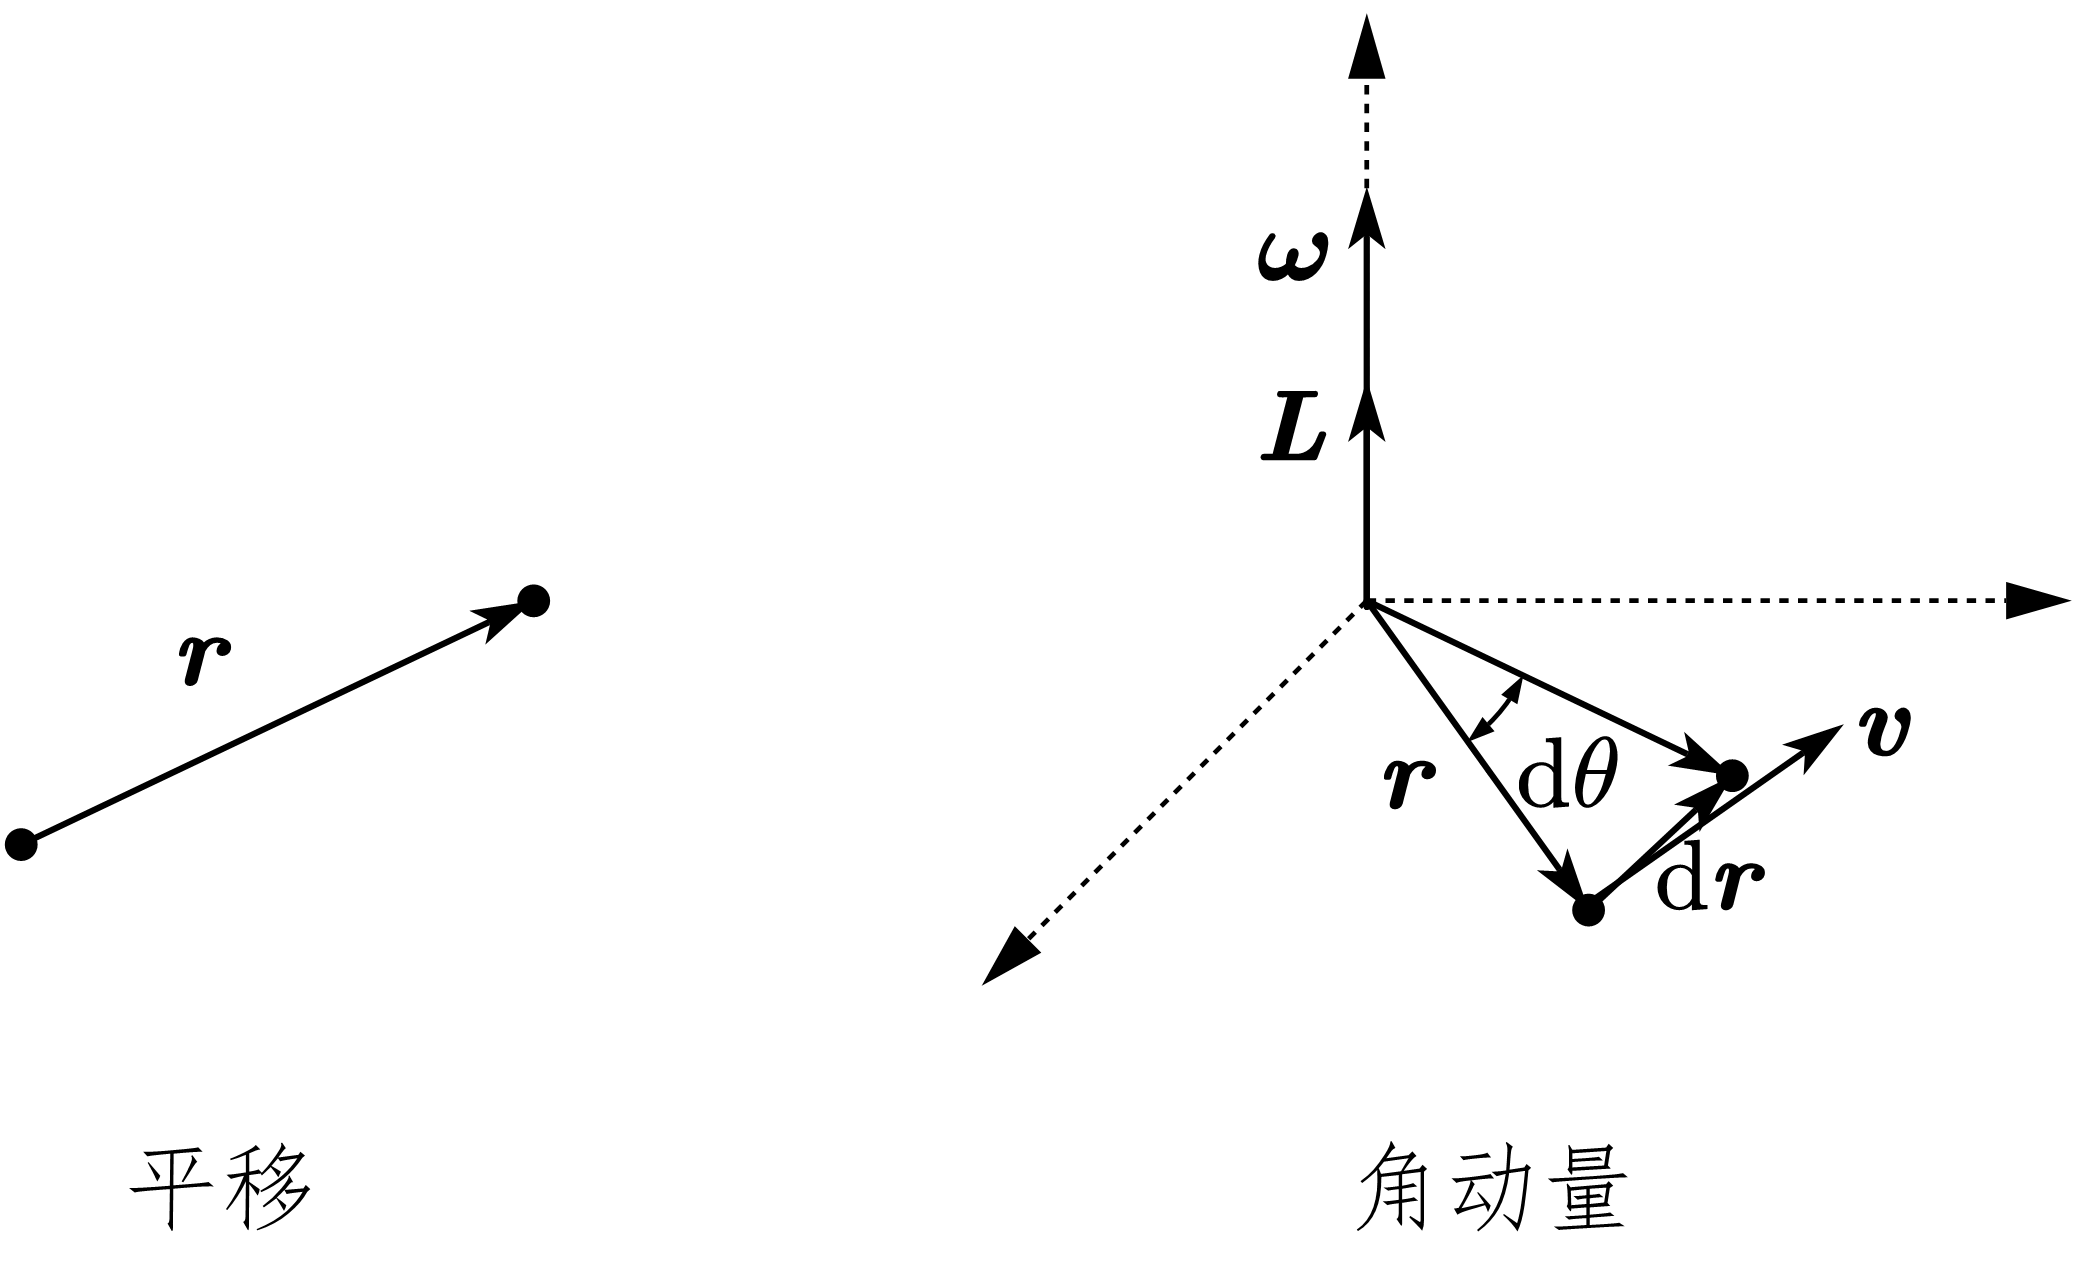
\includegraphics[width=6cm]{figure/move-in-space.png}
\end{center}

\subsubsection{抛体运动}
如下图所示,考虑炮弹的运动轨迹。

\begin{center}
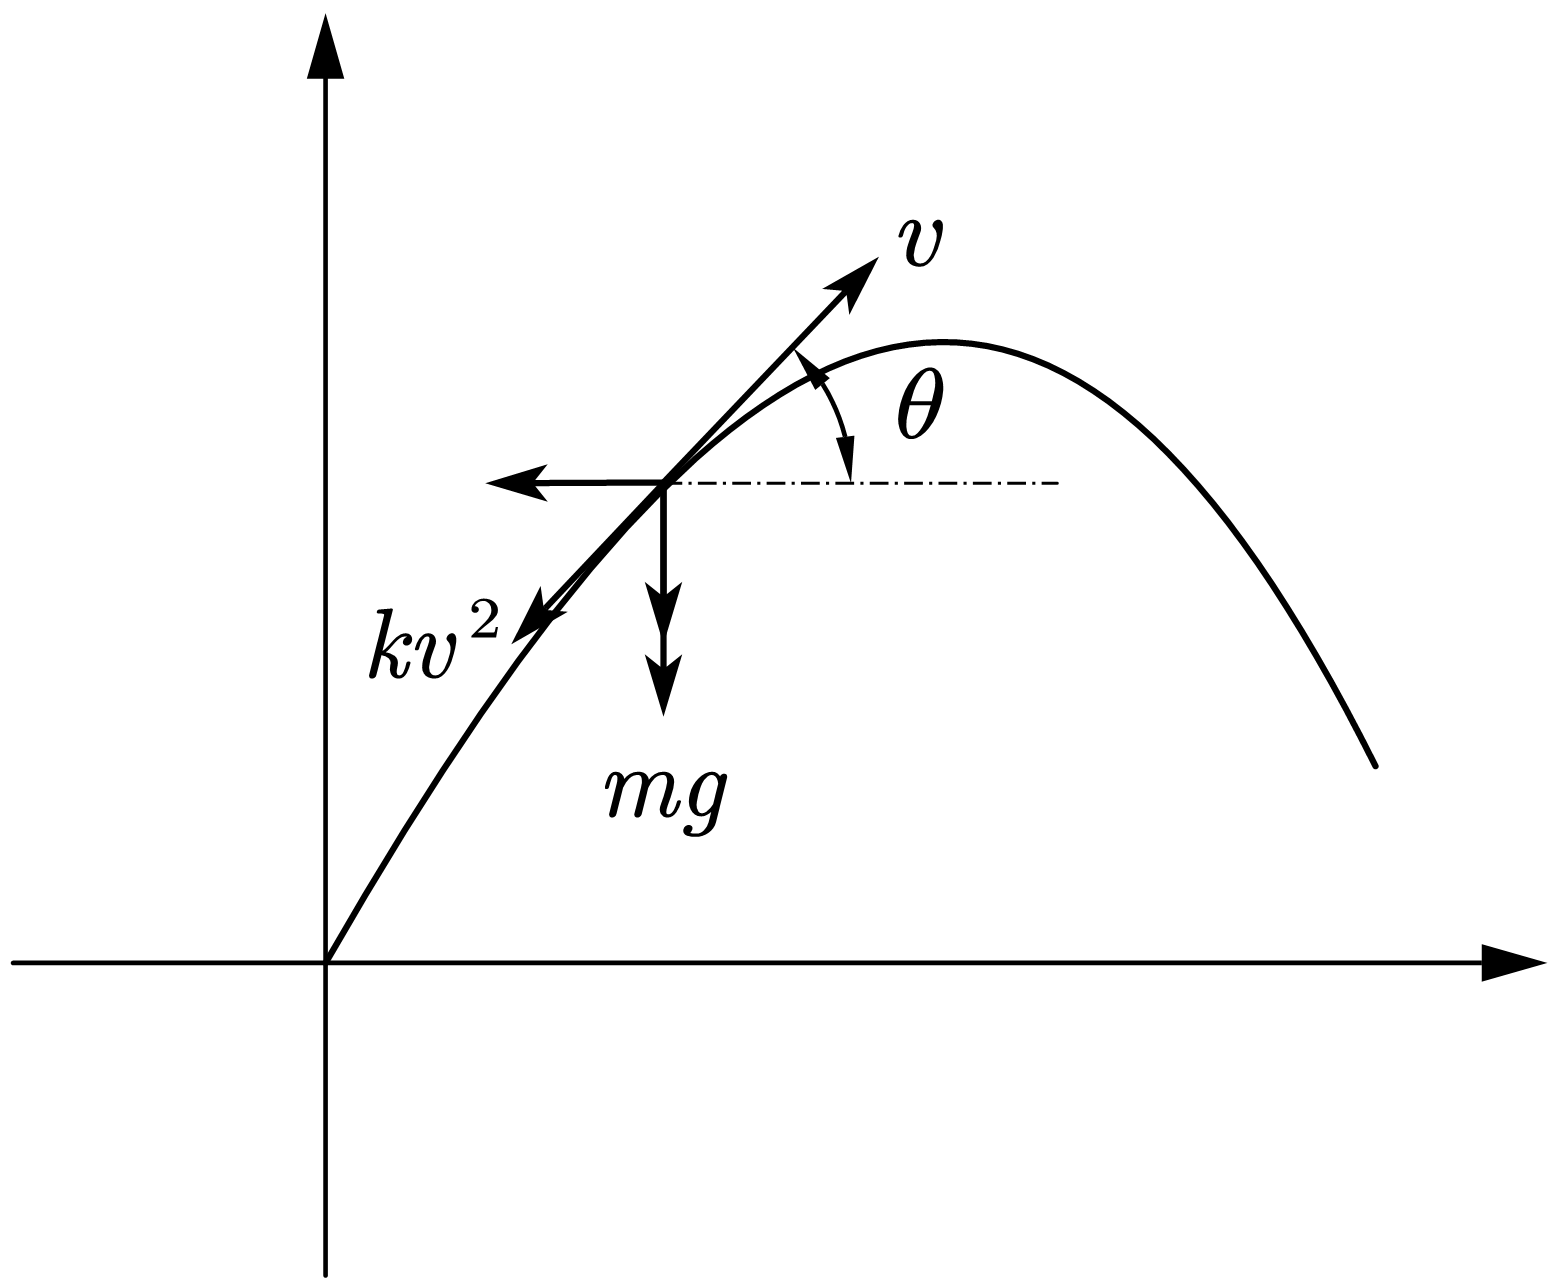
\includegraphics[width=6cm]{figure/projectile.png}
\end{center}

$f=kv^2$为阻力。$v$为速率。首先有速度方程:
\begin{empheq}{align}
\dot{x}&=v\cos\theta\\
\dot{y}&=v\sin\theta
\end{empheq}
然后有加速度方程:
\begin{empheq}{align}
\ddot{x}&=\odv{v\cos\theta}{t}=\dot{v}\cos\theta-\dot{\theta}v\sin\theta=-kv^2\cos\theta/m\\
\ddot{y}&=\odv{v\sin\theta}{t}=\dot{v}\sin\theta+\dot{\theta}v\cos\theta=-kv^2\sin\theta/m-g
\end{empheq}
这两个方程可以解出$\dot{v},\dot{\theta}$,最后得到4个方程:
\begin{empheq}[left=\empheqlbrace]{align}
\dot{v}&=-g\sin\theta-kv^2/m\\
\dot{\theta}&=-g\cos\theta/v\\
\dot{x}&=v\cos\theta\\
\dot{y}&=v\sin\theta\\
x(0)&=y(0)=0,v(0)=v_0,\theta(0)=\theta_0
\end{empheq}
实际上只有前2个方程是独立的。


\subsection{形变}

\subsection{碰撞}

\subsection{振动}

\section{拉格朗日力学}
\subsection{最小作用量原理与拉格朗日函数}
\subsubsection{最小作用量原理}


\subsubsection{拉格朗日函数的性质}
\paragraph*{可缩放}

\paragraph*{可加性}

\paragraph*{拉格朗日函数不唯一}

\paragraph*{惯性参考系}

\paragraph*{伽里略相对性原理}
\subsubsection{守恒律}
守恒律是拉格朗日函数的特殊性质。

\paragraph*{能量守恒}

\paragraph*{动量守恒}

\paragraph*{角动量守恒}

\subsection{各种情形下的拉格朗日函数}
\subsubsection{势场中的质点系}


\section{哈密顿力学}

